\documentclass[a4paper]{report}
\usepackage[margin=1.5in]{geometry}

\usepackage[utf8]{inputenc}
\usepackage[T1]{fontenc}
\usepackage{textcomp}
\usepackage[spanish]{babel}
\decimalpoint

\usepackage{csquotes}
\usepackage[sorting=none]{biblatex}
\addbibresource{refs.biblatex}

\usepackage{amsmath, amssymb}
\usepackage{amsthm}
\usepackage{bm}
\usepackage{braket}

\usepackage{graphicx}

\usepackage{hyperref}
\hypersetup{
    colorlinks,
    citecolor=red,
    filecolor=black,
    linkcolor=blue,
    urlcolor=black
}

\usepackage[marginal]{showlabels}

\DeclareMathOperator{\R}{\mathbb{R}}
\DeclareMathOperator{\C}{\mathbb{C}}
\DeclareMathOperator{\N}{\mathbb{N}}
\DeclareMathOperator{\Z}{\mathbb{Z}}
\DeclareMathOperator{\F}{\mathbb{F}}

\let\H\relax
\DeclareMathOperator{\H}{\mathcal H}
\DeclareMathOperator{\Sz}{\mathcal S}

\DeclareMathOperator{\dom}{Dom}
\DeclareMathOperator{\prob}{Prob}
\DeclareMathOperator{\id}{id}
\DeclareMathOperator{\Tr}{Tr}
\DeclareMathOperator{\tr}{tr}
\DeclareMathOperator{\Op}{Op}
\DeclareMathOperator{\W}{W}
\DeclareMathOperator{\Fr}{\mathcal{F}\!}

\newtheorem{definition}{Definición}
\newtheorem{theorem}{Teorema}
\newtheorem{proposition}{Proposición}
\newtheorem{lemma}{Lema}
\newtheorem{corollary}{Corolario}
\newtheorem{example}{Ejemplo}
\newtheorem{axiom}{Postulado}
\newtheorem{remark}{Observación}

\hfuzz=50pt

\title{Funciones de Wigner en el Espacio de Fase Discreto}
\author{Ernesto Camacho Ramírez}

\begin{document}
  \maketitle

  \tableofcontents

  \chapter{Introducción}

  El número de elementos de un conjunto general de
  operadores cuánticos unitarios sobre estados de $n$-qudit
  generalmente crece exponencialmente con $n$. Una excepción
  importante a ésta regla involucra el conjunto de
  operadores de Clifford que actúan sobre estados
  estabilizadores. Éstos estados juegan un papel importante
  en la corrección de errores cuánticos
  \cite{gottesmanHeisenbergRepresentationQuantum1998} y son
  cerrados bajo la acción de las compuertas de Clifford. La
  simulación eficiente de dichos sistemas con una
  computadora clásica se demostró con el algoritmo tableau
  de Aaronson y Gottesman \cite{
    aaronsonImprovedSimulationStabilizer2004,
  gottesmanHeisenbergRepresentationQuantum1998} para qubits
  ($d=2$). La busqueda de un explicación de por qué un
  algoritmo tan eficiente es posible para la simulación de
  circuitos de Clifford ha sido un objeto de mucho estudio
  \cite{gottesmanFaultTolerantQuantumComputation1999,
    howardContextualitySuppliesMagic2014,
  mariPositiveWignerFunctions2012}. El progreso reciente ha
  sido resultado del trabajo de Wooters
  \cite{woottersWignerFunctionFormulationFiniteState1987},
  Eisert \cite{mariPositiveWignerFunctions2012}, Gross
  \cite{grossHudsonTheoremFinitedimensional2006} y Emerson
  \cite{howardContextualitySuppliesMagic2014}, quienes han
  formulado una nueva perspectiva basada en los espacios de
  fase discretos de estados y operadores en espacios de
  Hilbert finitos, utilizando funciones discretas de Wigner.
  Se ha demostrado que los estados estabilizadores tienen
  funciones de Wigner discretas definidas positivas y que
  los operadores de Clifford son mapeos definidos positivos.
  Esto implica que los circuitos de Clifford son simulables
  eficientemente en computadores clásicas. En sistemas de
  dimensiones impares, se ha demostrado que los estados
  estabilizadores son análogos discretos a los estados
  gaussianos en sistemas continuos
  \cite{grossHudsonTheoremFinitedimensional2006} y se ha
  demostrado que las compuertas del grupo de Clifford tienen
  Hamiltonianos armónicos subyacentes que conservan los
  puntos discretos del espacio de fase
  \cite{kociaSemiclassicalFormulationGottesmanKnill2017}.
  Esto significa que los circuitos de Clifford se pueden
  expresar mediante integrales de trayectoria truncadas en
  el orden $\hbar^{0}$ y por lo tanto son expresamente
  clásicos
  \cite{kociaSemiclassicalFormulationGottesmanKnill2017,
  kohComputingQuopitClifford2017}.

  En este trabajo, buscamos construir, de una manera
  explícita, los operadores \textit{puntuales} de fase
  discretos (núcleos de la transformación de Wigner) para
  qubits y qutrits. Estrictamente hablando, buscamos la
  construcción \textit{estándar}
  \cite{woottersWignerFunctionFormulationFiniteState1987} y
  \textit{no estandar} (contribución del trabajo) de los
  núcleos que permitan dos formas de la función de Wigner,
  utilizando conjuntos de bases no equivalentes bajo
  transformaciones unitarias. La motivación para realizar
  éste trabajo es que, los núcleos que no son equivalentes
  conservan la propiedad tomográfica básica, lo que permite
  expresar la función de Wigner de cualquier estado como una
  combinación lineal de probabilidades medidas y la
  inequivalencia conduce a la posibilidad de encontrar
  estados no estabilizadores con funciones de Wigner no
  negativas, lo que contrasta con resultados previos para el
  caso discreto
  \cite{grossHudsonTheoremFinitedimensional2006,
  galvaoDiscreteWignerFunctions2005,
  cormickInterferenceDiscreteWigner2006}.

  \chapter{Preliminares}

  Para poder estudiar la función de Wigner discreta es
  necesario presentar la función de Wigner en el caso
  continuo. Para ésto requerimos un conocimiento básico de
  la mecánica cuántica, la cual es una teoría física que
  nació debido a la incapacidad de la mecánica clásica de
  explicar algunos fenómenos físicos que se observaban a
  nivel atómico. A diferencia de la mecánica clásica, la
  teoría cuántica es naturalmente probabilística y sus
  formulaciones matemáticas son bastante distintas. En la
  mecánica clásica, cuando se fija un estado de un sistema
  físico, el valor especificado por un observable (algo se
  puede medir del sistema) está completamente determinado.
  En la mecánica cuántica ésto ya no es cierto, los
  observables solo nos brindan distribuciones de los
  posibles valores. Antes de plantear los principios de la
  mecánica cuántica, repasamos rápidamente el concepto del
  espacio de fase en la mecánica clásica, ya que hay una
  relación directa de la distribución de Wigner con ambas
  teorías físicas.

  \section{La mecánica clásica y el espacio de fase}

  El concepto del espacio de fase es una herramienta de la
  mecánica clásica, la cual describe la evolución temporal
  de un sistema físico. Dicho de una manera muy sencilla, la
  mecánica clásica estudia partículas y sus trayectorias,
  las cuales se rigen de acuerdo a las leyes de Newton.  Se
  considera que la partícula se `mueve' en un espacio
  euclideano, es decir, su \textit{posición} está dado por
  $\bm{x} = (x_1,\ldots,x_n) \in \R^{n}$. El
  \textit{momentum} es una cantidad dada por $p_j = m \dot
  x_j$, donde $\bm{\dot x}$ es la derivada respecto al
  tiempo de la posición, es decir, la velocidad de la
  partícula, y $m$ es la \textit{masa} de la partícula. Las
  cantidades que uno desea medir de nuestro sistema físico
  se les llama \textit{observables}, y en la mecánica
  clásica, son las funciones continuas que tienen como
  argumentos las cantidades $\bm{x},\bm{p}$ y $m$. Ejemplos
  de ellos son el momentum, la energía cinética, la energía
  potencial, etc. La función de energía más usual es la que
  está dada como la suma de la \textit{energía cinética} y
  \textit{energía potencial}:
  \begin{equation}
    H(\bm{x},\bm{p})
    = \frac{1}{2m} \sum_{j=1}^{n} p_j^2 + V(x).
  \end{equation}
  A la energía del sistema se le conoce como el
  \textit{Hamiltoniano}.  Utilizando ésta función de
  energía, la ley de Newton nos brinda las ecuaciones de
  movimiento de la partícula en cuestión:
  \begin{equation}
    \frac{dx_j}{dt}
    = \frac{\partial H}{\partial p_j},
    \quad
    \frac{dp_j}{dt}
    = -\frac{\partial H}{\partial x_j}.
  \end{equation}
  Expresada como un sistema de ecuaciones diferenciales, a
  la ley de Newton se le conoce como las \textit{ecuaciones
  de Hamilton}.  

  Con ésto, es natural representar el estado del sistema
  clásico considerando el par $(x,p) \in \R^{2n}$. Al
  espacio $\R^{2n}$ se le conoce como el \textit{espacio de
  fase}. A las soluciones de las ecuaciones de Hamilton se
  les conoce como \textit{trayectorias}, y son curvas que
  viven en el espacio de fase.
  \begin{definition}
    El espacio de fase de una partícula que se mueve en
    $\R^{n}$ es $\R^{2n}$, considerado como el conjunto de
    las $(2n)$-tuplas de la forma
    \[
      \left(
        x_1, \ldots, x_n, p_1, \ldots, p_n
      \right),
    \] 
    donde $x_j$ y $p_j$ son elementos de $\R$.
  \end{definition}

  Cabe mencionar que el tratado moderno de la mecánica
  clásica está fundamentado en la geometría diferencial de
  las variedades simplécticas
  \cite{mcinerneyFirstStepsDifferential2013}, en donde el
  espacio de fase se define como el espacio cotangente del
  espacio de configuraciones $T^{*} \R_x \cong \R_x \times
  \R_p$, donde el espacio de configuraciones  $\R_x$ es el
  espacio de posición y el $\R_p$ es el espacio del
  momentum.  Para nuestros objetivos basta con desginar el
  espacio de fase como el espacio $\R^{2n}$.

  Notemos que por el momento no ha surgido ninguna
  interpretación probabilística en la mecánica clásica, pues
  es una teoría determinística. Dado que la teoría cuántica
  es probabilística, es natural preguntarnos ¿qué
  características de la mecánica clásica serían deseables en
  la teoría cuántica? y ¿qué beneficios habría en hacer un
  vínculo entre la mecánica clásica y la cuántica?
  \cite{schroeckQuantumMechanicsPhase1996}, especialmente
  cuando sabemos que la teoría cuántica (y sus derivados) es
  nuestra teoría más precisa. Un esfuerzo por vincular las
  descripciones clásicas y cuánticas del mundo es la
  representación de Wigner-Weyl-Moyal de la mecánica
  cuántica.  Ésta es una formulación que intenta usar la
  noción del espacio de fase en la dinámica cuántica y la
  idea básica es la construcción de
  \textit{cuasi-distribuciones} real-valuadas que
  representan a los sistemas cuánticos.

  \section{La mecánica cuántica}

  La teoría cuántica ha tomado distintas direcciones despues
  de su concepción en los años viente y existen distintas
  formulaciones matematicamente equivalentes que surgieron
  despues de las teorias iniciales de Schrödinger (mecánica
  de ondas) y de Heisenberg (mecánica matricial).  La más
  común hoy en dia es la formulación en el espacio de
  Hilbert, la cual fue desarrollada de manera rigurosa por
  Von Neumann en 1932.  La segunda formulación más común,
  especialmente en la teoría cuantica de campos, es la
  formulación de la integral de trayectoria de Feynman
  desarrollada en 1948.  Otra formulación, de particular
  interés para nuestro trabajo, es la formulación en el
  espacio de fase, que tiene sus inicios en 1932 por Wigner,
  pero que solo fue desarrollada como una descripción
  completa de la mecánica cuántica despues de la segunda
  guerra mundial. 

  En cualquiera de las formulaciones, la mecánica cuántica
  como toda teoría física, permite el cálculo del
  comportamiento y las propiedades de sistemas físicos. Dado
  un sistema físico, se definen los \textit{observables}
  como las cantidades que podemos medir sobre el sistema,
  por ejemplo la temperatura de algún cuerpo. En la
  formulación de Schrödinger, a los sistemas físicos se le
  asocia un espacio de Hilbert separable. Los observables
  físicos son representados por los operadores auto-adjuntos
  definidos en algún subespacio del espacio de Hilbert. El
  estado de un sistema representa toda la información del
  sistema en algún momento y está dado por operadores
  auto-adjuntos que satisfacen ciertas condiciones
  adicionales. Cuando no hay incertidumbre sobre el estado
  en el que está el sistema, podemos representar el estado
  por un vector del espacio de Hilbert, y decimos que el
  sistema está en un estado puro.

  El ejemplo físico de mayor importancia para éste trabajo
  es el de una partícula moviendose en un espacio
  Euclideano. El espacio de Hilbert asociado a éste sistema
  generalmente es el espacio de las funciones
  cuadráticamente integrables $L^2(\R^{n})$. Los estados
  puros del sistema son los elementos de éste espacio y el
  operador correspondiente al observable de la posición de
  la partícula es el operador que multiplica una función por
  la coordenada. La mecánica cuántica nos dice que no
  podemos medir la posición exacta de una partícula en un
  estado arbitrario, lo único que podemos hacer es obtener
  la \textit{probabilidad} de encontrar a la partícula en
  algún subconjunto de $\R^{n}$.  Estadísticamente, nos
  interesa obtener el \textit{valor esperado} de la posición
  de la partícula en un estado en específico, así como el
  valor esperado de otros operadores de interés como lo son
  la energía del sistema, el momentum, el momentum angular,
  entre otros. La mecánica cúantica nos permite estudiar los
  sistemas y sus observables de manera probabilística y
  también nos permite describir su evolución temporal por
  medio de la ecuación de Schrödinger. 
  
  \subsection{La formulación en el espacio de Hilbert}

  Con lo anterior aclarado, comencemos definiendo los
  conceptos y algunos de los postulados que necesitaremos de
  la mecánica cuántica. No será necesario estudiar la
  evolución temporal del sistema. Para un repaso al análisis
  funcional, teoría de medida y algebra lineal que
  necesitaremos, el lector puede consultar el apéndice (?).

  \begin{axiom}
    A cada sistema cúantico le corresponde un espacio de
    Hilbert $\H$. Los estados del sistema son todos los
    operadores lineales $\rho : \H \to \H$,
    definidos-positivos y de traza finita, tales que $\Tr(
    \rho) = 1$.
  \end{axiom}

  Un estado cuántico $\rho$ se dice \textit{puro}, is
  existe un elemento $\psi \in \H$, tal que para todo
  $\alpha \in \H$ se cumple
  \[
    \rho(\alpha)
    = \frac{\braket{\psi | \alpha}}{\braket{\psi | \psi}}
    \psi
  \] 
  De ésta manera, cuando hablemos de un estado puro,
  podremos referirnos a un elemento $\psi \in \H$, algo que
  casi siempre sucede en la literatura física.

  \begin{axiom}
    A cada observable físico, $A$, sobre el espacio de fase
    clásico, le corresponde un observable cuántico
    representado por un operador auto-adjunto $\hat{A} :
    \mathcal D_{\hat{A}} \to \H$.  
  \end{axiom}

  Es importante aclarar que el dominio de un operador no es
  un detalle pequeño, ya que generalmente no están definidos
  en todo el espacio de Hilbert. Muchos problemas surgen del
  ignorar los detalles de los dominios.

  \begin{axiom}
    La probabilidad que una medición de una observable $A$ 
    sobre un sistema en el estado $\rho$ de un
    resultado en el conjunto de Borel $E \subset \R$ está
    dado por
    \[
      \mu_{\rho}^{A}(E)
      = \Tr\left( P_A(E) \circ \rho \right)
    \] 
    donde el mapa $P_A : \mathcal B(\R) \to \mathcal L(\H)$,
    es la medida proyección valuada con el mapa $A$ dado por
    el teorema espectral.
  \end{axiom}

  El teorema espectral nos dice que para cualquier operador
  auto-adjunto $A$, existe una medida
  proyección-valuada $P_{A}$ tal que $A$ puede
  ser representado por la integral
  \[
    A
    = \int_{\R} \lambda dP_{A}(\lambda).
  \] 
  Para operadores de espacios de dimensión finita ésto se
  reduce a la diagonalización de la matrices Hermíticas.

  Si un sistema cuántico está en un estado descrito por un
  vector unitario $\psi \in \H$, entonces el valor esperado
  de un observable $A$ satisface
  \[
    \langle \hat{A} \rangle_\psi
    := \langle \psi, \hat{A}\psi \rangle,
  \] 
  donde $\langle \cdot, \cdot \rangle$ es el producto
  interno del espacio de Hilbert en cuestion. De manera
  general, dado un estado $\rho$, el valor esperado de
  un observable $\hat{A}$ está dado por
  \[
    \Tr\left(\hat{A}\rho\right)
    = \Tr\left( \rho\hat{A} \right),
  \]
  donde $\Tr$ es la traza del operador.

  
  \subsection{Los operadores de posición y de momentum}

  Los dos operadores indispensables para éste trabajo son
  los operadores de posición y de momentum. En particular
  pensemos en el sistema de una partícula moviendose en el
  espacio euclideano de dimensión $n$. El espacio de Hilbert
  es $L^2(\R^{n})$. Si $f \in L^2(\R^{n})$ es un vector
  unitario, entonces $|f|^2$ puede ser interpretado como la
  densidad de probabilidad de la posición de la partícula en
  el estado $f$, es decir, que la probabilidad de que la
  partícula se encuentre en el subconjunto $B \subset R^{n}$
  es $\int_B |f|^2$. 

  Con ésto identificamos a los operadores $Q_1,\ldots,Q_n$ 
  correspondientes a funciones coordenadas clásicas
  $q_1,\ldots,q_n$. En partícular, si $E \subset \R$ 
  entonces la probabilidad de que la $j$-ésima coordenada
  $x_j$ de la partícula se encuentre en $E$ está dada por
  \[
    \int_{x_j \in E} |f(x)|^2 \, dx.
  \] 
  Por lo tanto la medida proyección-valuda $\Pi_j$ para
  dicho observable será dada por
  \[
    \Pi_j(E) = 
    \text{la multiplicación por la función característica de
    } \{x : x_j \in E\},
  \] 
  y se sigue que el operador 
  \[
    Q_j = \int \lambda d\Pi_j(\lambda)
  \] 
  es la multiplicación por la $j$-ésima función coordenada,
  generalmente denotado por $X_j$, 
  \[
    Q_jf(x) = X_jf(x) = x_jf(x),
  \] 
  definido para todo $f \in L^2(\R^{n})$ tal que $x_jf \in
  L^2(\R^{n)}$.

  Notemos que no existen estados $f \in L^2(\R^{n})$ para
  los cuales los observables $Q_j$ tienen valores
  definitivos. Las eigenfunciones de los $Q_j$ son las
  deltas de Dirac $\delta_{x_0}(x) = \delta(x - x_0)$. Éstas
  se pueden considerar como un conjunto de estados `estados
  idealizados' y que forman una `base ortonormal continua'
  \[
    \langle \delta_{x_1}, \delta_{x_2} \rangle
    = \int \delta(x-x_1)\delta(x-x_2) \, dx
    = \delta(x_1-x_2),
  \] 
  \[
    f = \int f(x)\delta_x \, dx
    = \int \langle f, \delta_x \rangle \delta_x \, dx,
  \] 
  donde las integrales se interpretan en el sentido de
  distribuciones.


  .

  Informalmente, los eigenvectores del operador de posición
  forman un conjunto completo de vectores, es decir, podemos
  expandir cualquier estado $\ket \psi$ en los eigenvectores de
  posición. La relación de completitud es
  \[
    \id_{\H}
    = \int_{\R} \ket x \bra x \, dx, 
  \] 
  y así podemos representar a $\ket \psi$ como
  \begin{equation}
    \ket \psi
    = \id_{\H} \ket \psi
    = \int_{\R} \ket x \bra x \ket \psi \, dx
    = \int_{\R} \psi(x) \ket x \, dx
  \end{equation}
  donde $\psi(x)$ es la \textit{función de onda} 
  \begin{equation}
    \psi(x)
    = \braket{x|\psi},
  \end{equation}
  del estado $\ket \psi$ en el \textit{espacio de posición}.
  Similarmente podemos expresar el estado $\ket \psi$ 
  respecto a los eigenvectores del operador de momentum
  utilizando la relación de completitud:
  \[
    \id_{\H}
    = \int_{\R} \ket p \bra p \, dp.
  \] 
  Analogamente, ésto nos brinda
  \begin{equation}
    \ket \psi
    = \int_{\R} \ket p \bra p \ket \psi \, dp
    = \int_{\R} \psi(p) \ket p \, dp,
  \end{equation}
  donde la función onda en el \textit{espacio de posición}
  es
  \begin{equation}
    \psi(p)
    = \braket{p|\psi}.
  \end{equation}
  Las funciones $\psi(x)$ y $\psi(p)$ son dos
  representaciones del \textit{mismo} estado $\ket \psi$.
  Más adelante veremos que la transformada de Fourier
  conecta la función de posición $\psi(x)$ con la del
  momentum $\psi(p)$, 
  \begin{equation}
    \psi(x)
    = \frac{1}{\sqrt{2\pi\hbar}} \int_{\R} \psi(p)e^{ixp /
    \hbar} \, dp.
  \end{equation} 

  \subsection{En dimensión finita}

  \chapter{Función de Wigner}

  \section{Mecánica cuántica en el espacio de fase}

  El principio de la incertidumbre hace que el concepto de
  un espacio de fase de la mecánica cuántica, análogo al de
  la mecánica clásica, sea problemático. Ésto se debe a que
  la posición y el momentum de una partícula no ésta bien
  definida de manera simultánea, así que no se puede definir
  una densidad de probabilidad conjunta verdadera. Aún así
  exiten funciones que se \textit{asemejan} a distribuciones
  sobre el espacio de fase, llamadas funciones de
  distribución quasi-probabilísticas, las cuales son útiles
  de manera práctica, además de vincular de cierta manera a
  la mecánica clásica y la cuántica. Ésto sucede porque
  dichas quasi-distribuciones nos permiten calcular los
  valores esperados de los operadores cuánticos de manera
  muy similar a los promedios clásicos de la mecánica
  estadística. La primera y más conocida de éstas funciones
  es la cuasi-distribución ó función de Wigner.

  La función de Wigner tiene una larga historia que inicia
  con un artículo publicado por Eugene P. Wigner en 1932
  \cite{wignerQuantumCorrectionThermodynamic1932} sobre
  correcciones cuánticas del equilibrio termodinámico. La
  idea principal de Wigner fue introducir una
  quasi-distribución que le permite calcular valores
  esperados cuánticos de una manera análoga a los valores
  esperados de la mecánica estadística. Para el caso de un
  de una función $\psi$ la expresión que expuso Wigner
  originalmente (para una dimensión) es:
  \begin{equation}
    \label{eqn:wigners_original}
    W(x,p)
    = \frac{1}{\hbar \pi} \int_{\R}
    \overline{\psi(x+y)}\psi(x-y) e^{\frac{2i}{\hbar}py} \,
    dy.
  \end{equation}
  En el caso de un estado cuántico puro, la función $W(x,p)$
  representa al estado $\psi$ de manera análoga a una
  densidad probabilística sobre el espacio de fase. Wigner
  partió de la mecánica estadística clásica, la cual nos
  dice que cuando se tiene un conjunto de partículas, la
  evolución del sistema puede ser estudiado de manera
  probabilística mediante la ecuación de Liouville, la cual
  nos brinda una distribución sobre el espacio de fase [?].
  La idea es considerar una distribución en el espacio de
  fase que nos permita hacer las mismas interpretaciones
  probabilísticas de la mecánica cuántica que podemos hacer
  con la formulación en el espacio de Hilbert.

  Unos años antes de la publicación de Wigner, Hermann Weyl
  formuló una manera de mapear observables clásicos a
  observables cuánticos, lo cual se conoce como la
  cuantización de Weyl [?]. Debido a la no conmutatividad de
  los operadores canónicos $\hat{x}$ y $\hat{p}$, la
  cuantización de un observable clásico no es único y es
  necesario introducir un orden específico. Para el mapeo de
  Weyl, el orden utilizado para los operadores canónicos se
  conoce como el orden simétrico, por ejemplo $xp \mapsto
  \frac{1}{2}\left( \hat{x} \hat{p} + \hat{p} \hat{x}
  \right)$, ésto nos permite mapear polinomios de los
  operadores canónicos a operadores lineales sobre algún
  espacio de Hilbert. Generalizando, Weyl utiliza la la
  transformación de Fourier, para producir operadores
  correspondientes a ciertas funciones de $x$ y $p$ en el
  espacio de fase que satisfacen algunas condiciones de
  regularidad. Existe una relación directa entre los mapeos
  de Weyl y de Wigner que presentaremos más adelante. 

  Utilizando las transformaciones de Wigner y de Weyl,
  Enrique Moyal y Groenewold formularon una descripción
  completa de la mecánica cuántica en el espacio de fase, de
  manera independiente
  \cite{curtrightQuantumMechanicsPhase2012}.  El trabajo de
  Groenewold (en forma de su tésis de 1946) reconoció que el
  mapeo de Weyl es realmente una transformación invertible,
  y \textit{no} solo una regla de cuantización
  \cite{todorovQuantizationMystery2012}. Por otro lado Moyal
  desarrolló sus ideas sobre la naturaleza estadística de la
  mecánica cuántica, y en su formulación se introduce un
  producto en el espacio de fase correspondiente al producto
  de operadores en el espacio de Hilbert, tal producto se le
  conoce como el producto-$\star$ ó producto de Moyal. Ésta
  tercera formulación de la mecánica cuántica, en especial
  la representación de estados cuánticos en el espacio de
  fase, ha sido muy útil en muchas ramas de la física,
  particularmente en la óptica cuántica [?].

  \section{Transformación de Wigner}

  Para fines de nuestro trabajo no es necesario dar un
  recuento completo de la mecánica cuántica en el espacio de
  fase, en caso de que el lector esté interesado en la
  formulación completa de la mecánica cuántica en el espacio
  de fase, le invtamos a consultar los trabajos de Moyal [?]
  y Groenwold [?]. Lo que haremos es definir la
  transformación de Wigner para ciertas funciones, lo que
  nos permitirá definir la función de Wigner de un estado
  cuántico. Para ésto primero introducirimos el concepto de
  la cuantización de Weyl con la finalidad de dar argumentos
  ligeramente más rigurosos que aquellos que generalmente se
  encuentran en varios trabajos y libros de física.

  Consideremos un conjunto de partículas que se mueven en un
  esapcio $\R^{n}$. La ecuación de Liouville rige la
  evolución temporal de una función de distribución en el
  espacio de fase del conjunto de partículas [WIKI]. La
  solución de dicha ecuación nos brinda una densidad
  probabilística y dado un observable $A : \R^{2n} \to \R$,
  que depende de la posición $x$ y del momentum $p$ de una
  partícula, podemos calcular el valor esperado del
  observable como
  \begin{equation}
    \mathbb E[A]
    = \iint A(x,p) F(x,p) \, dx \, dp,
  \end{equation}
  donde $F$ es la densidad de probabilidad de Liouville. La
  densidad $F$ contiene toda la información del
  \textit{conjunto} de partículas, es decir del sistema. La
  intención es poder calcular valores esperados de
  observables cuánticos de manera análoga, es decir,
  mediante una integración en el espacio de fase, en donde
  la densidad que obtenemos representa a algún estado
  cuántico:

  \begin{equation}
    \Tr\left(\hat{\rho} \hat{A}\right)
    = \iint A(x,p)W(x,p) \, dx \, dp,
  \end{equation}

  La función $W : \R^{2n} \to \R$ que actúa como una
  distribución probabilística es precisamente la
  transformación de Wigner de un estado cuántico.
  Desafortunadamente no es una distribución verdadera, pues
  puede tomar valores negativos (de aquí proviene la
  asignación de \textit{quasi}-distribución). Sin embargo,
  nos permite calcular los valores esperados de los
  operadores cuánticos y otras cantidades probabilísticas
  como las densidades de la posición y momentum de la
  partícula, dandonos una representación de nuestro estado
  cuántico distinta y útil.

  Notemos que la definición (\ref{eqn:wigners_original}) es
  una transformación integral de una función $\psi \in
  L^2(\R^{n})$. Para poder definir la transformación de un
  estado cuántico $\hat{\rho}$, tendremos que tomar algunos
  pasos previos. En particular introducimos el concepto de
  \textit{cuantización} lo que nos permite pasar de un
  observable clásico definido en el espacio de fase a un
  operador cuántico.

  \subsection{La transformación de Weyl}

  El problema de la cuantización consiste en encontrar una
  correspondencia entre funciones sobre el espacio de fase
  $\R^{2n}$ y operadores auto-adjuntos sobre $L^2(\R^{n})$,
  tales que las propiedades de los observables clásicos se
  reflejen lo más posible en sus correspondientes
  observables cuánticos, en una manera consistente con la
  interpretación probabilística de la mecánica cuántica.
  Dada la no conmutatividad de los operadores de posición y
  de momentum, no hay una correspondencia única, por lo
  tanto se restringe el mapeo de una manera ad-hoc, buscando
  satisfacer ciertas propiedades razonables. Por ejemplo es
  deseable que las funciones coordenadas de posición y de
  momentum $x_j$ y $p_j$ correspondan a los operadores
  $\hat{x}_j$ y $\hat{p}_j$, así como el operador
  correspondiente a la función constante $1$ debe ser el
  operador identidad, entre otros.  A pesar de que no hay un
  manera única de cuantizar observables clásicos, existe una
  que es más \textit{natural}, conocida como la cuantización
  de Weyl. 

  La idea de la cuantización de Weyl, es la siguiente:
  consideramos un observable clásico $A : \R^{2n} \to \R$,
  comunmente llamado \textit{símbolo} en el análisis
  armónico y en la óptica cuántica, y lo expresamos mediante
  la transformación de Fourier inversa:
  \begin{equation}
    A(x,p)
    = \frac{1}{(2\pi\hbar)^{n}} \int_{\R^{2n}} \Fr A(\xi,
    \eta) e^{\frac{i}{\hbar} \left( \xi x + \eta p\right) }
    \, d\xi \, d\eta,
  \end{equation}
  donde $\Fr A$ es la transformada de Fourier de $A$.
  Enseguida reemplazamos de manera formal a las variables
  $x$ y $p$ por los operadores $\hat{x}$ y $\hat{p}$, (ésto
  corresponde con el orden simétrico de Weyl) para obtener
  al operador $\hat{A}$ correspondiente:
  \begin{equation}
    \label{eqn:weyl_quant_1}
    \hat{A}(\hat{x},\hat{p})
    = \frac{1}{(2\pi\hbar)^{n}} \int_{\R^{2n}} \Fr
    A(\xi,\eta) e^{\frac{i}{\hbar} \left( \xi \hat{x} + \eta
    \hat{p}\right) } \, d\xi \, d\eta.
  \end{equation}
  Para darle un sentido riguroso a la integral es necesario
  pedir ciertas condiciones de regularidad a la función $A$.
  En la literatura matemática generalmente se comienza por
  definir la transformación de Weyl sobre el espacio de las
  funciones rápidamente decrecientes $\Sz(\R^{2n}) \subset
  L^2(\R^{2n})$ y luego se extiende a las funciones
  cuadraticamente integrables y por dualidad a las
  distribuciones templadas $\Sz'(\R^{2n})$. Omitiremos las
  pruebas de extensión, pero para darle sentido riguroso
  comenzamos por definir al operador exponencial que aparece
  en el integrando de (\ref{eqn:weyl_quant_1}).
  \begin{definition}
    El operador $\hat{M}(\xi, \eta) : L^2(\R^{n}) \to
    L^2(\R^{n})$ definido como
    \begin{equation*}
      \hat{M}(\xi,\eta)
      = e^{\frac{i}{\hbar} \left( \xi \hat{x} + \eta \hat{p}
      \right) }
      = e^{-\frac{i}{2\hbar} \xi \eta} e^{\frac{i}{\hbar}
      \eta \hat{p}} e^{\frac{i}{\hbar} \xi \hat{x}}
      = e^{\frac{i}{2\hbar} \xi \eta} e^{\frac{i}{\hbar}
      \xi \hat{x}} e^{\frac{i}{\hbar} \eta \hat{p}},
    \end{equation*} 
    se conoce como el operador característico de Moyal
    (entre otros nombres). Actúa sobre alguna función $\psi
    \in L^2(\R^{n})$ de la siguiente manera:
    \begin{equation}
      \hat{M}(\xi,\eta)\psi(x)
      = e^{\frac{i}{2\hbar} \xi\eta} e^{\frac{i}{\hbar} \xi
      x} \psi(x + \eta).
    \end{equation}
  \end{definition}
  Utilizando la definición del operador $\hat{M}(\xi,\eta)$,
  se puede dar una definición rigurosa de la transformación
  de Weyl sobre el espacio de Schwartz:
  \begin{definition}
    Sea $A \in \Sz(\R^{2n})$. El operador de Weyl, $\hat{A}
    = \Op_W(A)$ del símbolo $A$ se define para $\psi \in
    \Sz(\R^{n})$ como
    \begin{equation}
      \label{eqn:weyl_quant_2}
      \hat{A}\psi(x)
      = \frac{1}{(2\pi\hbar)^{n}}
      \int_{\R^{2n}} \Fr A(\xi,\eta) \hat{M}(\xi,\eta)
      \psi(x) \, d\xi \, d\eta.
    \end{equation}
  \end{definition}
  Es más común expresar a la transformación de Weyl en términos
  del símbolo $A$ directamente, sin recurrir a la
  transformada de Fourier. Utilizando la definición de $\Fr$,
  de manera formal tenemos:
  \begin{align*}
    \Op_W(A)
    &= \frac{1}{(2\pi\hbar)^{n}} \int_{\R^{2n}} \Fr
    A(\xi,\eta)\hat{M}(\xi,\eta) \, d\xi \, d\eta \\
    &= \frac{1}{(2\pi\hbar)^{n}} \int_{\R^{2n}} \left(
    \int_{\R^{2n}} A(x,p)e^{-i(\xi x + \eta p)} \, dx \, dp
    \right) \hat{M}(\xi,\eta) d\xi \, d\eta \\
    &= \frac{1}{(2\pi\hbar)^{n}} \int_{\R^{2n}} A(x,p) \left(
    \int_{\R^{2n}} e^{-i(\xi x + \eta p)} \hat{M}(\xi,\eta)
    \, d\xi \, d\eta \right) \, dx \, dp \\
    &= \frac{1}{(2\pi\hbar)^{n}} \int_{\R^{2n}} A(x,p)
    \Delta(x,p) \, dx \, dp.
  \end{align*} 
  El la literatura matemática, el operador $\Delta(x,p)$ se
  conoce como el operador de Grossmann-Royer y generalmente
  se denota $\hat{R}(\xi,\eta)$. En la literatura física
  comunmente se llama el operador puntual de cuantización,
  en donde formalmente se puede ver como la transformada de
  Fourier del operador de Weyl $\hat{M}(\xi,\eta)$,
  \begin{equation}
    \label{eqn:phase_point_operator}
    \Delta(x,p)
    = \int_{\R^{2n}} e^{-i(\xi x + \eta p)}
    \hat{M}(\xi,\eta) \, d\xi \, d\eta.
  \end{equation}
  Extendiendo las definiciones anteriores a las
  distribuciones templadas, resulta que el operador puntual
  es la cuantización de Weyl de la medida de Dirac $\delta_x
  \otimes \delta_p \in \Sz'(\R^{2n})$ concentrada en el
  punto $(x,p)$. La acción del operador puntual sobre un
  elemento de $\Sz(\R^{2n})$ está dado de la siguiente
  manera.


  \begin{definition}
    El operador de Heisenberg-Weyl $\hat{T}(\xi,\eta)$ se
    define como
    \[
      \hat{T}(\xi,\eta)\psi(x)
      = e^{\frac{i}{\hbar} (\eta x - \frac{1}{2} \eta
      \xi)}\psi(x - \xi).
    \] 
    Equivalentemente
    \[
      \hat{T}(\xi,\eta)\psi(x)
      = e^{\frac{i}{\hbar} \sigma((\xi,\eta),
      (\hat{x},\hat{p}))}\psi(x),
    \] 
    donde $\sigma((x,p),(x',p')) = p \cdot x' - p' \cdot x$.
    El operador de Heisenberg-Weyl satisface las relaciones
    \[
      \hat{T}(z_0)\hat{T}(z_1)
      = e^{\frac{i}{\hbar} \sigma(z_0,z_1)}
      \hat{T}(z_1)\hat{T}(z_0),
    \] 
    y
    \[
      \hat{T}(z_0+z_1)
      = e^{-\frac{i}{2\hbar} \sigma(z_0,z_1)}
      \hat{T}(z_0)\hat{T}(z_1).
    \] 
  \end{definition}
  \begin{definition}
    El operador de Grossmann-Royer $\hat{R}(\xi,\eta)$ es el
    operador
    \[
      \hat{R}(\xi,\eta) : \Sz(\R^{n}) \to \Sz(\R^{n})
    \] 
    definido por las formulas 
    \[
      \hat{R}(0,0)\psi(x)
      = \psi(-x),
    \]
    y
    \[
      \hat{R}(\xi,\eta)
      = \hat{T}(\xi,\eta) \hat{R}(0,0)
      \hat{T}(\xi,\eta)^{-1},
    \] 
    donde $T$ es el operador de Heisenberg-Weyl. El operador
    de Grossmann-Royer es unitario y es una involución en el
    espacio de Schwartz. Su acción sobre cualquier función
    $\psi : \R^{n} \to \C$ está dado por
    \[
      \hat{R}(\xi,\eta)\psi(x)
      = e^{\frac{2i}{\hbar} \eta (x - \xi)}\psi(2\xi - x).
    \] 
  \end{definition}
  El operador de Heisenberg-Weyl y de Grossmann-Royer están
  relacionados por medio de la transformada de Fourier
  simpléctica, i.e.,
  \[
    \hat{R}(\xi,\eta)\psi(x)
    = \frac{1}{2^{n}} F_\sigma(\hat{T}(\cdot)\psi(x)](-z_0).
  \] 
  \begin{definition}
    El operador puntual de cuantización $\Delta(x,p)$
    (operador de Grossmann-Royer) es un operador acotado de
    la forma
    \begin{equation}
      \label{eqn:point_operator}
      \Delta(x,p)
      = 2e^{-2i x p} V(2x)U(-2x) P
      %= \hat{R}(\xi,\eta)\psi(x)
      %= e^{\frac{2i}{\hbar} \eta \cdot (x - \xi)} \psi(2\xi
      %- x).
    \end{equation} 
    donde $V = e^{ix \hat{x}}$ y $U = e^{ix \hat{p}}$ son
    subgrupos del grupo de Weyl y $P$ es el operador de
    paridad definido como $(P\psi)(x) = \psi(-x)$.  Su
    acción sobre un elemento $\psi \in \Sz(\R^{2n})$ está
    dado por
    \begin{equation}
      \label{eqn:grossmann_royer_op}
      \left(\Delta(x,p)\psi\right)(y)
      = 2e^{2i p (y-x)}\psi(2x - y)
    \end{equation}
  \end{definition}
  El operador puntual de cuantización es unitario sobre
  $L^2(\R^{n})$, pero no es de clase traza. Utilizando al
  operador de Grossmann-Royer podemos definir el operador de
  Weyl en términos del símbolo $A$ directamente.
  
  \begin{definition}
    Sea $A \in \Sz(\R^{2n})$. El operador de Weyl $\hat{A} =
    \Op_W(A)$ está dado para todo $\psi \in \Sz(\R^{n})$ 
    como
    \begin{equation}
      \left( \hat{A}\psi \right)(x)
      = \frac{1}{(\pi\hbar)^{n}} \int_{\R^{2n}}
      A(\xi,\eta)\hat{R}(\xi,\eta)\psi(x) \, d\xi \, d\eta,
    \end{equation}
    donde $\hat{R}(\xi,\eta)$ se conoce como el operador de
    Grossmann-Royer.
  \end{definition}

  Expresando en términos del observable $A$ nos permite
  representar al operador de Weyl de forma integral.
  Utilizando la definición de $\hat{R}(\xi,\eta)$ tenemos
  \[
    \hat{A}\psi(x)
    = (\pi\hbar)^{-n} \int_{\R^{2n}} A(\xi,\eta)
    e^{\frac{2i}{\hbar} \eta \cdot (x - \xi)} \psi(2\xi - x)
    \, d\xi \, d\eta,
  \] 
  y luego aciendo el cambio de variable $y = 2\xi - x$,
  obtenemos
  \begin{equation}
    \label{eqn:weyl_quant_k}
    \hat{A}\psi(x)
    = (2\pi\hbar)^{-n} \int_{\R^{2n}} e^{\frac{i}{\hbar} p
    \cdot (x - y)} A\left( \frac{x+y}{2}, p \right) \psi(y)
    \, dy \, dp.
  \end{equation}
  No todos los operadores se pueden expresar de forma
  integral, los que sí, se llaman operadores integrales y
  son de la forma
  \[
    \hat{A}\psi(x) = \int_{\R^{n}} K(x,y) \psi(y) \, dy
  \] 
  donde $K$ se conoce como el \textit{núcleo
  (distribucional)} de $\hat{A}$. Observando el integrando
  de la ecuación (\ref{eqn:weyl_quant_k}), podemos ver que
  para un operador de Weyl, el núcleo está dado por
  \begin{equation}
    K(x,y)
    = (2\pi\hbar)^{-n} \int_{\R^{n}} e^{\frac{i}{\hbar} p
    \cdot (x - y)}A\left( \frac{x+y}{2}, p \right) \, dp.
  \end{equation}
  Podemos invertir ésta relación por medio de la fórmula de
  inversión de Fourier y otro cambio de variable, para
  obtener una expresión para el símbolo $A$ en términos del
  núcleo $K$ del operador,
  \begin{equation}
    A(x,p)
    = \int_{\R^{n}} e^{-\frac{i}{\hbar} p \cdot y} K\left( x
    + \frac{1}{2}y, x - \frac{1}{2}y\right) \, dy.
  \end{equation}
  Ésto nos permite transformar un operador que admite una
  representación integral a un símbolo que es integrable en
  el espacio de fase. Al símbolo obtenido a partir de
  operador de Weyl se conoce como símbolo de Weyl. Lo
  anterior nos dice que existe una correspondencia entre el
  símbolo de Weyl y los núcleos distribucionales de los
  operadores de Weyl. Más aún, existe una biyección entre
  los símbolos cuadracticamente integrables sobre el esapcio
  de fase y una clase de operadores acotados de
  $L^2(\R^{n})$ conocidos como los operadores
  Hilbert-Schmidt.

  Gosson demuestra que la definición que hemos dado de la
  transformación de Weyl se puede extender a las
  distribuciones templadas del espacio de fase,
  específicamente, 
  \[
    \Op_W : \Sz'(\R^{2n}) \to \mathcal
    L(\Sz(\R^{n}),\Sz'(\R^{n})),
  \]
  donde $\mathcal L(\Sz(\R^{n}),\Sz'(\R^{n}))$ es el espacio
  de los operadores continuos del espacio de Schwartz a su
  dual. Además, utilizando el triplete de Gel'fand
  \[
    \Sz(\R^{2n})
    \subset L^2(\R^{2n})
    \subset \Sz'(\R^{2n}),
  \]
  Gosson demuestra en partícular que la transformación de
  Weyl de una función cuadraticamente integrable corresponde
  a un operador Hilbert-Schmidt. Ésto es particularmente
  útil para nosotros porque los estados cuánticos
  representados por operadores de densidad son de
  Hilbert-Schmidt.

  En resumen tenemos una manera de cuantizar observables
  clásicos, que brinda operadores cuánticos que satisfacen
  varias propiedades útiles, por ejemplo nos brinda los
  operadores correctos correspondientes a las funciones
  coordenadas
  $x_j$ y $p_j$:
  \begin{equation}
    \Op_W(x_j)\psi = x_j\psi,
    \quad
    \Op_W(p_j)\psi = -i\hbar \partial_{x_j}\psi.
  \end{equation}
  Con la transformación de Weyl definida, pasamos a definir
  la transformación de Wigner para el caso continuo y luego
  mostramos la relación entre las dos transformaciones.
  Dicha relación nos permite extender la transformación de
  Wigner a las distribuciones templadas de manera rigurosa.

  La cuestión de la \textit{decuantización} no es trivial.
  Una fuente de los posibles problemas es que para muchos
  operadores de Weyl de observables clásicos es dificil
  identificar si son de clase traza. Ésto es importante
  porque generalemente se denota la decuantización de
  operadores de Weyl mediante
  \[
    A(x,p)
    = \Tr\left( \Delta(x,p) \Op_W(A) \right). 
  \] 
  Pero dicha expresión es problemática por no tiene sentido
  para todo observable $A$. De hecho la traza solo existe de
  manera obvia cuando $\Op_W(A)$ es de clase traza.

  

  

  \subsection{La transformación de Wigner}

  Lo que sigue está principalmente basado en los libros de
  Gosson \cite{gossonWignerTransform2017} y de Folland
  \cite{follandHarmonicAnalysisPhase1989}, quienes
  introducen la función de Wigner de manera general, como
  una transformación integral entre ciertos espacios de
  funciones. Iniciamos definiendo una versión más general de
  la transformación de Wigner, la cual se conoce como la
  \textit{transformación de Wigner cruzada}. 

  \begin{definition}
    La transformación de Wigner cruzada es una
    transformación integral
    \[
      W : L^2(\R^{n}) \times L^2(\R^{n}) \to L^2(\R^{2n}),
    \]
    definida como
    \begin{equation}
      \label{eqn:cross_wigner_transform}
      W(\psi,\phi)(x,p)
      = (2\pi\hbar)^{-n} \int_{\R^{n}} e^{-\frac{i}{\hbar} p
      \cdot y} \psi(x + \tfrac{1}{2}y) \overline{\phi(x -
      \tfrac{1}{2}y)} \, dy,
    \end{equation}
    para $\psi, \phi \in L^2(\R^{n})$ y $x,p \in \R^{n}$.  
  \end{definition}
  En partícular, denotaremos la transformación de Wigner de
  un elemento $\psi$ de $L^2(\R^{n})$ como $W\psi =
  W(\psi,\psi)$. Gosson demuestra que la transformación de
  Wigner cruzada puede ser extendida a un mapeo sesquilineal
  sobre las distribuciones templadas, $W : \Sz'(\R^{n})
  \times \Sz'(\R^{n}) \to \Sz'(\R^{2n})$. Por ejemplo, la
  transformación de Wigner de la delta de Dirac es
  \[
    W\delta = (2\pi\hbar)^{-n} (\delta \otimes 1).
  \] 
  Utilizando los operadores puntuales (operador de
  Grossmann-Royer) nos permite dar una definición
  particularmente sencilla de la transformación de Wigner:
  \begin{definition}
    Sean $\psi,\phi \in \Sz(\R^{n})$. La función
    $(\psi,\phi) \mapsto W(\psi,\phi)$ definida como
    \begin{equation}
      W(\psi,\phi)(x,p)
      = \frac{1}{(\pi\hbar)^{n}} \langle \hat{R}(x,p)\psi,
      \overline{\phi} \rangle_{gosson}
      = \frac{1}{(\pi\hbar)^{n}} \langle \phi,
      \hat{R}(x,p)\psi \rangle.
    \end{equation}
  \end{definition}
  La transformación de Wigner cruzada satisface varias
  propiedades interesantes, enunciamos algunas de ellas.
  \begin{itemize}
    \item Es real valuada.
    \item Es acotada y continua para $\psi,\phi \in
      L^2(\R^{n})$.
    \item Tiene ciertas propiedades de traslación.
    \item \ldots
  \end{itemize}
  \begin{proposition}
    Si $\psi, \phi \in L^2(\R^{n})$, entonces $W(\psi,\phi)
    = \overline{W}(\phi,\psi)$. En particular
    \[
      W\psi
      = W(\psi,\psi)
      = \overline{W}(\psi,\psi)
      = \overline{W\psi},
    \] 
    por lo tanto $W\psi$ es real-valuada. 
  \end{proposition}

  Tiene varias propiedades de traslación interesantes. 
  \begin{proposition}
    Para todo $\psi \in L^2(\R^{n})$ y $z_0 = (x_0,p_0) \in
    \R^{2n}$ tenemos
    \[
      W(\hat{T}(z_0)\psi, \hat{T}(z_0)\phi)(z)
      = T(z_0)W(\psi,\phi)(z),
    \] 
    donde $T(z_0)$ es una traslación, $z \mapsto z + z_0$, y
    sobre funciones definidas en $\R^{2n}$ actúa como
    $T(z_0)f(z) = f(z-z_0)$.
  \end{proposition}
  
  \begin{proposition}
    Sean $\psi \in L^2(\R^{n})$ y supongamos que $W\psi \in
    L^{1}(\R^{2n})$. Entonces $W\psi \in L^{1}(\R^{2n})$ y
    \begin{equation}
      \int_{\R^{2n}} (W\psi)(x,p) \, dx \, dp 
      = \|\psi\|^2_{L^2(\R^{n})}.
    \end{equation}
  \end{proposition}

  \begin{proposition}
    Supongamos que $\psi, \phi \in L^2(\R^{n})$. La función
    $z \mapsto W(\psi,\phi)(z)$ es acotada y continua en
    $\R^{2n}$.
  \end{proposition}

  \begin{proposition}
    Sean $\psi,\phi \in \Sz'(\R^{n})$. La función $z
    \mapsto W(\psi,\phi)(z)$ es continua en $\R^{2n}$.
  \end{proposition}

  \begin{proposition}
    La transformación de Wigner cruzada satisface la
    identidad de Moyal, en particular
    \begin{equation}
      \|W\psi\|_{L^2(\R^{2n})}
      = (2\pi\hbar)^{-n / 2} \|\psi\|_{L^2(\R^{n})}.
    \end{equation}
  \end{proposition}

  \begin{proposition}
    Supongamos que $\psi, \phi \in L^{1}(\R^{n}) \cap
    L^2(\R^{n})$. Entonces
    \begin{equation}
      \int_{\R^{n}} W(\psi,\phi)(x,p) \, dp
      = \psi(x)\overline{\phi}(x),
    \end{equation}
    \begin{equation}
      \int_{\R^{n}} W(\psi,\phi)(x,p) \, dx
      = \Fr\psi(p) \overline{\Fr\phi}(p).
    \end{equation}
    En particular tenemos
    \begin{equation}
      \int_{\R^{n}} W\psi(x,p) \, dp
      = |\psi(x)|^2,
      \quad
      \int_{\R^{n}} W\psi(x,p) \, dx
      = |\Fr\psi(p)|^2.
    \end{equation}
  \end{proposition}

  Gosson menciona que las dos fórmulas anteriores solo son
  casos particulares de una transformación de Radon
  (generalizada) de la distribución de Wigner $W\psi$,
  correspondiente a una integración sobre planos
  Lagrangianos particulares $\ell_P = 0 \times \R^{n}$ y
  $\ell_X = \R^{n} \times 0$, respectivamente. En general
  uno puede definir dicha transformación por medio de
  \[
    R_{\ell}(u)
    = \int_{\ell} W\psi(z) d\mu_{\ell}(z)
  \] 
  donde $d\mu_{\ell}(z)$ es la medida euclideana sobre el
  plano Lagrangiano $\ell$. Un tratado riguroso se puede
  encontrar bajo el área de la geometría integral.

  De las proposiciones anteriores ya podemos ver la utilidad
  que nos puede brindar la transformación de Wigner, ya que
  por medio de integrales sobre algún eje podemos recuperar
  las supuestas densidades de la posición y momentum de las
  funciones de onda. Aún con éste primer acercamiento, no
  hemos hablado sobre la transformación de Wigner de estados
  cuánticos ya sean puros o mixtos, ni de operadores en
  general. Para ésto nos conviene definir la transformación
  de Weyl, la cual nos permitirá asociar observables
  clásicos en el espacio de fase con operadores lineales de
  un espacio de Hilbert.

  Consideremos el operador de Weyl de un observable adecuado
  sobre el espacio de fase. Entonces podemos utilizar a la
  transformación cruzada de Wigner para calcular el producto
  interior $\langle \psi, \hat{A}\phi \rangle$, para
  funciones de Schwartz.
  \begin{proposition}
    \label{prop:wigner-weyl}
    Sea $A \in \Sz(\R^{2n})$. Tenemos que
    \begin{equation}
      \langle \psi, \hat{A}\phi \rangle
      = \int_{\R^{2n}} A(x,p)W(\psi,\phi)(z) \, dx \, dp.
    \end{equation}
    para todo $\psi, \phi \in \Sz(\R^{n})$, donde $\hat{A} =
    \Op_W(A)$.
  \end{proposition}
  De hecho, Gosson menciona que muchas veces se define la
  transformación de Wigner $W$ mediante el producto interno
  anterior. Utilizando ésto, finalmente podemos expresar el
  valor esperado de un operador de Weyl en un estado $\psi$
  mediante una integral en el espacio de fase.
  \begin{proposition}
    El valor esperado de un operador de Weyl $\hat{A} =
    \Op_W(A)$ en un estado $\psi$ está dado por
    \begin{equation}
      \langle \hat{A} \rangle_\psi
      = \frac{1}{\langle \psi, \psi \rangle} 
      \int_{\R^{2n}} A(z) W\psi(z) \, dz.
    \end{equation}
  \end{proposition}  

  Con las propiedades que se probaron en la sección de la
  transformación de Wigner respecto a la integración en los
  ejes del espacio de fase, y con el resultado anterior que
  nos permite calcular el valor esperado de un operador de
  Weyl con la transformación de Wigner, podemos formular
  parte de la mecánica cuántica en el espacio de fase.

  \subsection{Análisis armónico cuántico}

  Recordemos que el operador de densidad describe el
  conjunto estadístico de estados cuánticos puros. En
  general un estado cuántico es un operador que nos brinda
  una distribución de las posibles mediciones de algún
  observable en un experimento. El estado cuántico puro
  coincide con la noción de información completa del
  sistema. Como hemos mencionado antes, generalmente se
  identifica a los estados puros con los elementos del
  espacio de Hilbert $\H$ en cuestión, matemáticamente los
  estados puros se identifican con proyección ortogonales
  $\Pi_\psi$ sobre el rayo $\C \psi = \{\lambda \psi :
  \lambda \in \C\}$. Generalmente se denota la proyección
  utilizando la notación Dirac y en ocasiones la
  adoptaremos:
  \[
    \ket{\psi}\bra{\psi} := \Pi_\psi. 
  \] 
  En la práctica no conocemos la información completa del
  sistema y en éste caso decimos que el sistema está en un
  \textit{estados mixtos}. Podemos definir un estado mixto
  como un conjunto de pares $\{(\lambda_j,\psi_j)\}_{j \in
  \N}$ donde $\psi_j \in L^2(\R^{n})$ es un estado puro y
  $0 \leq \lambda_j \leq 1$ es un probabilidad clásica, es
  decir, $\sum_j \lambda_j = 1$. Con ésto identificamos al
  estado mixto con la suma de proyectores
  \[
    \hat{\rho} = \sum_{j}^{} \lambda_j \Pi_j.
  \] 
  Al operador $\rho$ se le conoce como el operador de
  densidad. Es de clase de traza con $\Tr(\rho) = 1$. La
  \textit{distribución de Wigner} del operador de densidad
  es la función
  \[
    \rho = \sum_{j}^{} \lambda_j W\psi_j.
  \] 

  \begin{definition}
    Un estado cuántico es el conjunto de pares $(\lambda_j,
    \psi_j) \in [0,1] \times L^2(\R^{n})$, indexado por un
    conjunto discreto $F$ donde $\|\psi_j\|_{L^2(\R^{n})} =
    1$ para todo $j \in F$ y $\sum_{j \in F} \lambda_j = 1$.
    El operador lineal $\hat{\rho}$ sobre $L^2(\R^{n})$
    definido por
    \begin{equation}
      \hat{\rho} \psi
      = \sum_{j \in F}^{} \lambda_j \Pi_{\psi_j} \psi
      = \sum_{j \in F}^{} \lambda_j \langle \psi, \psi_j
      \rangle \psi_j,
    \end{equation}
    es el operador de densidad asociado al estado. La
    distribución de Wigner del estado es
    \begin{equation}
      \rho = \sum_{j \in F}^{} \lambda_j W\psi_j.
    \end{equation}
  \end{definition}
  El operador de densidad es auto-adjunto, semi-definido
  positivo, es de clase de traza con $\Tr(\hat{\rho}) = 1$.
  La serie $\rho = \sum_{j}^{} \lambda_j W\psi_j$, converge
  en $L^2(\R^{2n})$ y 
  \[
    \rho \in L^2(\R^{2n}) \cap L^{\infty}(\R^{2n}).
  \] 
  El espectro de un operador de densidad $\hat{\rho}$ sobre
  $L^2(\R^{n})$ es discreto y consiste de números no
  negativos tales que $\lambda_1 \geq \lambda_2 \geq \ldots
  \geq 0$, y $\lim_{j \to \infty} \lambda_j = 0$ (en el
  caso en que $F$ es infinito). Junto con los eigenvectores
  $\psi_j$ podemos expresar al operador como
  \[
    \rho \psi
    = \sum_{j}^{} \lambda_j \langle \psi, \psi_j \rangle
    \psi_j,
  \] 
  y su distribución de Wigner es
  \[
    \rho 
    = \sum_{j}^{} \lambda_j W\psi_j,
  \] 
  donde los $\psi_j$ son ortogonales. En particular notamos
  que distintos estados mixtos nos pueden brindar el mismo
  operador, Gosson menciona que el significado físico de
  ésta ambigüedad no está bien comprendida. Podemos decir
  que la información estadística del estado mixto está
  codificado en el operador de densidad de tal manera que
  podemos hacer predicciones sobre el estado que no dependen
  de la manera en que está expresado. 

  Existe una relación directa entre la distribución de
  Wigner de un operador de densidad por medio de la
  transformación de Weyl. El operador de densidad
  $\hat{\rho}$ puede ser expresado en términos de su
  distribución de Wigner:
  \begin{equation}
    \hat{\rho} 
    = (2\pi\hbar)^{n} \Op_W(\rho).
  \end{equation}

  Se puede demostrar que todo operador de clase traza es el
  producto de dos operadores Hilbert-Schmidt. Ahora
  consideremos en particular el caso en que los operadores
  se define por medio de su símbolo $\hat{A} = \Op_W(A)$.

  \begin{proposition}
    Sean $\hat{A} = \Op_W(a)$ y $\hat{B} = \Op_W(b)$
    operadores de Hilbert-Schmidt. Entonces
    \begin{equation}
      \Tr\left( \hat{A}\hat{B} \right) 
      = \Tr\left( \hat{B}\hat{A} \right) 
      = \frac{1}{(2\pi\hbar)^{n}} \int_{\R^{2n}} a(z)b(z) \,
      dz.
    \end{equation}
  \end{proposition}

  \begin{proposition}
    Sea $\hat{A} = \Op_W(a)$ un operador de clase de traza.
    Si adicionalmente $a \in L^{1}(\R^{n})$, entonces
    \begin{equation}
      \Tr\left( \hat{A} \right) 
      = \frac{1}{(2\pi\hbar)^{n}} \int_{\R^{2n}} a(z) \, dz.
    \end{equation}
  \end{proposition}

  Si $\psi \in L^2(\R^{n})$ es una función con norma
  unitaria, la información de $\psi$ es equivalente a la
  información de su transformación de Wigner [GOSSON]. Se
  puede probar que la proyección ortogonal $\hat{\Pi}_\psi$ 
  sobre el rayo $\{\lambda \psi : \lambda \C\}$ es el
  operador de Weyl con símbolo
  \[
    \pi_\psi = (2\pi\hbar)^{n}W\psi.
  \] 
  Con ésto podemos identificar un estado cuántico $\psi$ con
  su función de Wigner.

  \begin{definition}
    Consideremos el estado mixto $\{(\psi_j,\alpha_j)\}$,
    con $\|\psi_j\| = 1$, $\alpha_j \geq 0$ y $\sum_{j}^{}
    \alpha_j = 1$. El operador de densidad $\rho$ de
    éste estado es el operador de Weyl
    \begin{equation}
      \rho
      = (2\pi\hbar)^{n} \sum_{j}^{} \alpha_j \Op_W(W\psi_j).
    \end{equation}
    La transformación de Wigner de éste estado es la función
    \begin{equation}
      \rho = \sum_{j}^{} \alpha_j W\psi_j.
    \end{equation}
  \end{definition}

  Consideremos un operador de densidad $\hat{\rho}$,
  utilizando la fórmula () verificaremos que obtenemos, una
  expresión que coincide con la definición que hemos dado de
  la distribución de Wigner. Dado que la traza es
  independiente de la base ortonormal, utilizaremos la base
  de eigenvectores del operador de densidad:
  \begin{align*}
    \rho(x,p) &= \Tr\left( \hat{\rho} \Delta(x,p) \right) \\
              &= \sum_{j}^{} \langle \psi_j, 
              \Delta(x,p) \hat{\rho} \psi_j \rangle \\
              &= \sum_{j}^{} \langle \psi_j, \Delta(x,p)
              \sum_{k}^{} \lambda_k \Pi_{\psi_k} \psi_j
              \rangle \\
              &= \sum_{j}^{} \langle \psi_j, \Delta(x,p)
              \lambda_j \psi_j \rangle \\
              &= \sum_{j}^{} \lambda_j W\psi_j.
  \end{align*}

  \subsection{Gosson again}

  \begin{definition}
    Un operador de densidad sobre un espacio de Hilbert
    separable es un operador acotado $\hat{\rho} : \H \to
    \H$ tal que
    \begin{itemize}
      \item $\hat{\rho}$ es auto-adjunto y semi-definido
        positivo: $\hat{\rho} = \hat{\rho}^{*}, \hat{\rho}
        \geq 0$.
      \item $\hat{\rho}$ es de clase de traza y
        $\Tr(\hat{\rho}) = 1$.
    \end{itemize}
  \end{definition}

  El ejemplo más sencillo es el de un estado puro, $\psi \in
  \H$ tal que $\|\psi\| = 1$. Consideremos ahora el operador
  de proyección
  \[
    \hat{\rho}_\psi : \H \to \{\alpha \psi : \alpha \in
    \C\}.
  \] 
  Para todo $\phi \in \H$ tenemos
  \[
    \hat{\rho}_\psi \phi
    = \alpha \psi,
    \quad \alpha = \langle \psi, \phi \rangle.
  \] 
  El operador $\hat{\rho}_\psi$ es un operador de densidad
  puro asociado a $\psi$. Si $\H = L^2(\R^{n})$, entonces
  \[
    \hat{\rho}_\psi \phi(x)
    = \int_{\R^{n}} \overline{\psi}(y)\phi(y) \psi(x) \, dy,
  \] 
  por lo tanto el núcleo asociado a $\hat{\rho}_\psi$ es el
  producto tensorial
  \[
    K_{\hat{\rho}_\psi} = \psi \otimes \overline{\psi}.
  \] 
  Resulta que el operador de densidad puro $\hat{\rho}_\psi$ 
  es simplemente el operador de Weyl cuyo símbolo (salvo un
  factor) es simplemente la transformación de Wigner de
  $\psi$.

  \begin{proposition}
    Sea $\hat{\rho}_\psi$ un operador de densidad asociado a
    un estado puro $\psi$ por medio de la proyección.
    Entonces
    \begin{itemize}
      \item el símbolo de Weyl $\rho_\psi$ de
        $\hat{\rho}_\psi$ y la transformación de Wigner
        $W\psi$ de $\psi$ están relacionados por la fórmula
        \begin{equation}
          \rho_\psi(z)
          = (2\pi\hbar)^{n} W\psi(z).
        \end{equation}
      \item Si $\|\psi\|_{L^2(\R^{n})} = 1$ entonces el
        valor esperado $\langle \hat{A} \rangle_\psi$ de un
        operador de Weyl $\hat{A}$ está dado por
        \[
          \langle \hat{A} \rangle_\psi
          = (\frac{1}{2\pi\hbar})^{n} \Tr(\hat{\rho}_\psi
          \hat{A}).
        \] 
    \end{itemize}
  \end{proposition}

  En el caso en que no tenemos toda la información del
  estado del sistema, podemos formar una mezcla de estados
  $\psi_1,\psi_2,\ldots$ donde cada $\psi_j$ tiene una
  probabilidad $\alpha_j$ de ser el estado ``verdadero''.
  Entonces el operador de densidad del estado mixto es el
  operador auto-adjunto
  \[
    \hat{\rho}
    = \sum_{j}^{} \alpha_j \hat{\rho}_{\psi_j}j
  \] 
  donde $\sum_{j}^{} \alpha_j = 1$ y $\alpha_j \geq 0$.

  \begin{proposition}
    Sea $\hat{\rho} : L^2(\R^{n}) \to L^2(\R^{n})$ un
    operador de densidad. Entonces existe una familia
    $\{\psi_j\}_{j \in F}$ en $L^2(\R^{n})$ y una sucesión
    $\{\lambda_j\}_{j \in F}$ de números con $\lambda_j \geq
    0$ y $\sum_{j}^{} \lambda_j = 1$ tales que el símbolo de
    Weyl $\rho$ de $\hat{\rho}$ está dado por
    \[
      \rho 
      = \sum_{j}^{} \lambda_j W\psi_j.
    \] 
  \end{proposition}
  \begin{proof}
    Existen subespacio ortogonales entre si $\H_1,
    \H_2,\ldots$ de $L^2(\R^{n})$ tales que
    \[
      \hat{\rho}
      = \sum_{j}^{} \alpha_j \hat{\rho}_{\H_j},
      \quad 
      \sum_{j}^{} m_j \alpha_j = 1,
    \] 
    donde $\hat{\rho}_j$ es la proyección ortogonal de $\H$ 
    a $\H_j$ y $m_j = \dim \H_j$. Elige una base ortonormal
    $\psi_1,\ldots,\psi_{m_1}$ de $\H_1$, una base
    ortonormal $\psi_{m_1+1},\ldots,\psi_{m_1+m_2+1}$ de
    $\H_2$, etc. El símbolo de Weyl de $\hat{\rho}$ es
    \[
      \rho
      = \alpha_1 \sum_{j=1}^{m_1} W\psi_j
      + \alpha_2 \sum_{j=m_1}^{m_1+m_2+1} W\psi_j + \ldots.
    \] 
  \end{proof}

  \subsection{Integrando la función de Wigner sobre rectas}

  Una caracterización de la distribución de Wigner de un
  estado cuántico es que integrando sobre ciertos conjuntos
  del espacio de fase nos brinda las probabilidades de
  observar ciertos valores de ciertos observables. Ésto es
  una generalización de las densidades de posición y de
  momentum y se ha demostrado que la función de Wigner es la
  única que tiene ésta propiedad y por lo tanto es una que
  es deseable preservar.

  No es suficiente con obtener las marginales de la posición
  y de momentum correctas para poder determinar la
  distribución conjunta, pues hay más de una. En el espacio
  de fase, podemos integrar sobre franjas formadas por
  rectas paralelas y se puede demostrar que si tenemos un
  conjunto completo de éstas ``marginales'', podemos
  recuperar la distribución conjunta sobre todo el espacio.
  [Braasch] le llama a éste conjunto de marginales un
  conjunto tomograficamente completo.

  Como se ha mencionado anteriormente, integrando sobre $x$
  ó $p$ brinda las densidades de momentum ó de posición
  respectivamente. Un resultado más general nos dice que
  podemos integrar la función de Wigner sobre una franja
  definida por dos rectas paralelas $ax + bp = c_1$ y $ax +
  bp = c_2$ en el espacio de fase y obtener la probabilidad
  de observar un valor entre $c_1$ y $c_2$ del el operador
  de Weyl
  \[
    \Op_W(ax+bp) = a \hat{x} + b \hat{p}.
  \] 
  En lugar de usar la teoría espectral para operadores
  auto-adjuntos, utilizaremos la maquinaria de Dirac.
  [2201.05911] nos dice que $a \hat{x} + b \hat{p}$ es
  esencialmente auto-adjunto y su espectro es $\R$. Entonces
  por Dirac tenemos que $\ket r$ es una eigenvector
  generalizado de $a \hat{x} + b \hat{p}$ para cada $r \in
  \sigma\left( a \hat{x} + b \hat{p} \right) = \R$. 

  Ahora consideremos el mapeo unitario sobre las funciones
  de Schwartz
  \[
    U\psi(x) = e^{icx^2 / 2} \psi(x).
  \] 
  Notemos que $UPU^{-1} = Z = -c \hat{x} + \hat{p}$ para
  funciones de prueba. Tiene sentido pensar que $U$ 
  transforma los eigenvectores generalizados de $P$ a los de
  $Z$. Para cada $r \in \R$ la distribución
  \[
    e^{irx + icx^2 / 2}
  \] 
  es un eigenvector generalizado de $Z$. Los eigenvectores
  normalizados
  \[
    \frac{1}{\sqrt{2\pi}} e^{irx + icx^2 / 2}
  \] 
  forman un sistema ``$\delta$-completo''. Entonces la
  densidad de probabilidad de las amplitudes para $Z$ está
  dado por
  \[
    \braket{r|\psi}
    = \frac{1}{\sqrt{2\pi}} \langle e^{irx + i cx^2 / 2},
    \psi \rangle
    = \frac{1}{\sqrt{2\pi}} \int_{\R} e^{-irx-icx^2 /
    2}\psi(x) \, dx.
  \] 
  Y la densidad de probabilidad es
  \[
    D_Z(r)
    = \frac{1}{2\pi} \left|
    \braket{e^{irx+icx^2 / 2}|\psi}
    \right|^2.
  \] 
  Utilizando la teoría de medida [?] prueba que para todo
  estado $\ket \psi$, el push-forward $(x)_* \mathcal P_W =
  \mathcal P_{\hat{x}}$ donde $\mathcal P_W$ es la
  distribución dada por la densidad de Wigner del estado
  $\psi$ y $\mathcal P_{\hat{x}}$ es la distribución dada la
  densidad del operador de posición. En otras palabras, es
  simplemente el cálculo de las marginales.

  \begin{proposition}
    Para todo estado $\psi \in L^2(\R)$, la distribución de
    Wigner $\mathcal P_W$ es la única distribución sobre
    $\R^{2}$ tal que para todo número real $a$ y $b$, la
    ``distribución marginal'' $(ax+bp)_{*} \mathcal P_W$ es
    correcta en el sentido de que coincide con la
    distribución de probabilidad $\mathcal P_{a \hat{x} + b
    \hat{p}}$.
  \end{proposition}

  \section{Ejemplo: el oscilador armónico}

  Como ejemplo consideraremos el oscilador armónico de una
  partícula en una dimensión. El oscilador armónico es un
  modelo muy importante en un gran número de áreas de la
  física.  El Hamiltoniano asociado a éste sistema es
  \begin{equation}
    \hat{H}
    = \frac{\hat{p}^2}{2m} + \frac{m\omega^2}{2}
    \hat{x}^2,
  \end{equation}
  donde $m$ y $\omega$ son constantes positivas. El espectro
  del Hamiltoniano es discreto y resolviendo la ecuación
  independiente del tiempo obtenemos los eigenvalores y los
  eigenvectores. Introduciendo una constante para
  simplificar los cálculos
  \[
    a = \sqrt{\frac{\hbar}{m \omega}},
  \]
  obtenemos los niveles de energía
  \begin{equation}
    E_n
    = \hbar \omega \left( n + \frac{1}{2} \right),
    \quad n = 0,1,2,\ldots
  \end{equation}
  con sus correspondientes eigenvectores
  \begin{equation}
    \psi_n(x)
    = \frac{1}{\sqrt{2^{n} n! a \sqrt{\pi}}} e^{-x^2 / 2a^2}
    H_n(x),
    \quad n = 0, 1, 2,\ldots
  \end{equation}
  donde $H_n(x)$ es el $n$-ésimo polinomio Hermite.
  Como $H_0(x) = 1$, el estado ``de piso'' $\psi_0$ está
  dado por
  \[
    \psi_0(x)
    = \frac{1}{\sqrt{a \sqrt{\pi}}} e^{-x^2 / (2a^2)}.
  \]
  Utilizando la definición (\ref{eqn:wigners_original}), la
  función de Wigner para el estado $\psi_0$ está dado por
  \begin{align*}
    (W\psi_0)(x,p)
    &= \frac{1}{2\pi\hbar} \int_{\R} e^{-\frac{i}{\hbar} p y}
    \psi(x + \tfrac{1}{2}y) \overline{\psi(x -
    \tfrac{1}{2}y)} \, dy \\
    &= \frac{1}{2\pi\hbar} \int_{\R} e^{-\frac{i}{\hbar}py}
    \frac{1}{a\sqrt{\pi}}\exp\left( -\frac{x^2}{a^2} -
    \frac{y^2}{4a^2} \right)  \, dy \\
    &= \frac{1}{\pi\hbar} \exp\left( -\frac{a^2
    p^2}{\hbar^2} \right) \exp\left( -\frac{x^2}{a^2}
    \right). 
  \end{align*}
  Se puede demostrar que la función de Wigner
  correspondiente al $n$-ésimo eigenestado del oscilador
  armónico se puede expresar en términos del $n$-ésimo polinomio
  de Laguerre [CITE], 
  \[
    (W\psi_n)(x,p)
    = \frac{(-1)^{n}}{\pi} \exp\left[ -\left( \frac{x}{a}
    \right)^2 - \left( \frac{ap}{\hbar} \right)^2 \right]
    L_n\left[ 2\left( \frac{x}{a} \right)^2 + 2\left(
    \frac{ap}{\hbar} \right)^2 \right].
  \] 
  La figura (\ref{fig:harmonic_osc_wigner_3_7}) muestra la
  gráfica en el espacio de fase de las funciones de Wigner
  correspondientes a los estados $\psi_3$ y $\psi_7$.
  Notamos el incremento de oscilaciones de un estado a otro
  y la presencia de valores negativos.
  
  \begin{figure}[ht]
    \centering
    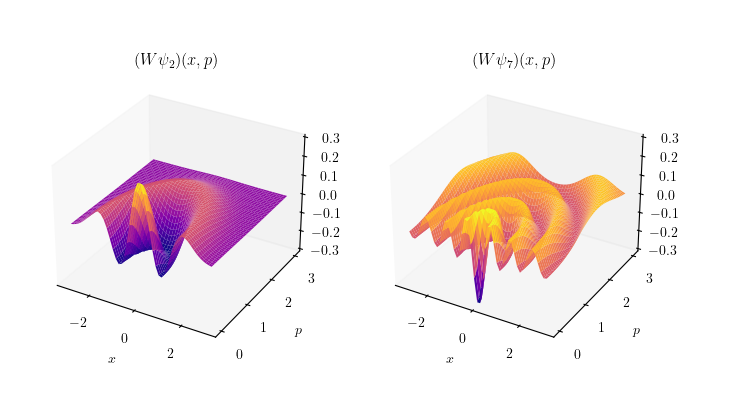
\includegraphics[width=1\textwidth]{
      imgs/harmonic_osc_wigner.png
    }
    \caption{Funciones de Wigner de los estados $\psi_3$ y
    $\psi_7$ del oscilador armónico, con $\hbar = 1$ y
    $\omega = 1$.}
    \label{fig:harmonic_osc_wigner_3_7}
  \end{figure}

  \chapter{Funciones de Wigner en el Espacio Fase Discreto}

  El objetivo de éste trabajo es construir dos versiones de
  la transformación de Wigner en el espacio discreto.

  Resumiendo el capítulo anterior, podemos representar a un
  estado cuántico por medio de la transformación de Wigner.
  A pesar de no ser una densidad sobre el espacio de fase,
  comparte varias propiedades, en particular nos permite
  calcular los valores esperados de ciertos observables
  cuánticos, en particular aquellos que su símbolo de Weyl
  está bien definido. Además podemos recuperar las
  densidades probabilísticas de la posición y del momentum
  itegrando la función de Wigner sobre el eje de momentum o
  de posición respectivamente. Ésta última característica
  solamente es un caso partícular de una propiedad más
  general de la función de Wigner.

  \section{Braasch}

  Para tener una versión análoga a la función de Wigner para
  el caso discreto, es necesario identificar que propiedades
  de la transformación en el caso continuo deseamos
  preservar.  Principalmente deseamos preservar (P1) el
  cálculo de los valores esperados de observables por medio
  de la integración sobre el espacio de fase, (P2) el de las
  marginales y (P3) el cálculo de probabilidades a lo largo
  de rectas en el espacio de fase.

  En la sección () se mostró que la distribución de Wigner
  satisface la siguientes propiedades:
  \begin{itemize}
    \item Realidad. Para todo $\hat{\rho}$, la distribución
      de Wigner $W(x,p)$ es real.
    \item Proyección. Para todo $\hat{\rho}$, al integrar a
      la distribuciónd e Wigner $W(x,p)$ sobre la linea $l =
      ax + bp$ en el espacio de fase nos brinda la
      probabilidad de medir $l$ del observable $a \hat{x} +
      b \hat{p}$.
    \item Hilbet-Schmidt producto interno. Para todo
      $\hat{\rho}_1$  y $\hat{\rho}_2$ se cumple que
      \[
        \Tr\left(\hat{\rho}_1 \hat{\rho}_2\right)
        = \int_{\R^{2n}} W_1(x,p) W_2(x,p) \, dx \, dp.
      \] 
    \item Traslación
  \end{itemize}

  Según [?], se puede expresar éstas propiedades en términos
  de los operadores puntuales. Los operadores puntuales
  $\Delta(x,p)$ deben ser auto-adjuntos, deben satisfacer
  las propiedades de ortogonalidad y al integrarlos sobre
  lineas en el espacio de fase nos deben de dar proyectores.

  \begin{itemize}
    \item $\hat{\Delta}(x,p)$ es auto-adjunto.
    \item ``Ortogonalidad''. 
      \[
        \Tr\left( \hat{\Delta}(x,p) \hat{\Delta}(x',p')
        \right)
        = \delta(x-x')\delta(p-p').
      \] 
    \item Supongamos que $\Pi_l$ es una proyección al
      eigenestado generalizado $a \hat{x} + b \hat{p}$ con
      eigenvalor, entonces
      \[
        \int_{\R^2} \delta(ax + bp - l) \hat{\Delta}(x,p) \,
        dx \, dp
        = \Pi_l.
      \] 
  \end{itemize}

  Existe un mapeo del espacio de Hilbert al espacio de fase
  que se puede interpretar como una cuasi-distribución
  conjunta sobre dos variables Fourier-conjugables. La idea
  es iniciar con un espacio de dimensión $N$, y resulta que
  hay distintas maneras de hacer ésta correspondencia.

  Schwinger desarrolló una base ortonormal de $N^2$ 
  operadores unitarios que forman una representación del
  grupo de Heisenberg-Weyl modulo su centro. Dado la base
  ortonormal de operadores, se puede describir al estado de
  un sistema utilizando los coeficientes de la expansión del
  operador de densidad en términos de la base. El trabajo
  consiste en elegir a la ``mejor'' base que resulte en las
  propiedades de la función de Wigner que deseamos
  preservar.  La idea de Wooters es construir una versión
  discreta de los operadores puntuales que preservan las
  propiedades. 

  Por otro lado, Hannay y Berry desarrollaron otro método
  donde la función de Wigner continua podía ser manipulada
  para definir una versión discreta sobre un látice $2N
  \times 2N$.

  Wootters, Galetti y de Toledo Piza y Cohendet hicieron
  investigaciones subsiguientes del caso $N \times N$.

  Hemos elegido el camino de Wootters. Empezando con la
  transformada de Fourier discreta y restringiendonos a
  dimensiones primas impares, podremos trabajar en analogía
  al caso continuo. El grupo de desplazamientos de
  Heisenberg-Weyl nos darán los operadores de paridad
  desplazados, los cuales se usarán para asignar puntos del
  espacio de fase a operadores.

  Un sistema cuántico con una espacio de Hilbert de
  dimensión $N$ será representado por un arreglo de $N
  \times N$ puntos. Los puntos $\alpha$ estarán dados por
  los pares $(a_1,a_2)$ de elementos de un campo finito
  $\Z_n$.

  Existe una base ortonormal de $N$ elementos para nuestro
  espacio de Hilbert, correspondientes a los eigenestados de
  algún observable. Denominemos a éste observable como la
  ``posición'' y diagramaticamente denotará el eje
  horizontal. Sus eigenvalores denotarán la coordenada del
  eje horizontal. Lo que sigue es identificar las lineas
  perpendiculares al eje horizontal del espacio de fase con
  los eigenestados que corresponden a los eigenvalores. El
  eje vertical será la variable Fourier-conjugada de la
  posición llamada el ``momentum''.

  Las propiedades marginales de la función de Wigner
  continua será fundamental en la construcción de la versión
  discreta. Una propiedad marginal consiste en un conjunto
  de resultados de sumas sobre lineas paralelas. Para el
  caso discreto, una linea se define como un conjunto de
  puntos $\alpha = (a_1,a_2)$ tales que $ma_1 + na_2 = p$ 
  donde $m, n, p \in \Z_N$. Las lineas son paralelas si
  tienen los mismos valores $m,n$ y solo difieren en $p$.
  Cada linea pertenece a un conjunto de $N$ lineas paralelas
  que se llamarán ``foliación'' o ``estriación''. La
  corerspondencia entre lineas y eigenestados existe debido
  a que ambos pertenecen a conjuntos de $(N+1)$ conjuntos de
  $N$ objetos.

  Ahora debemos introducir los operadores de desplazamiento.
  Fijando un conjunto de lineas al origen, un conjunto de
  lineas no paralelas pueden ser descritas por
  desplazamientos del origen. Denotamos $\hat{D}_\alpha =
  \hat{D}(a_1,a_2)$ para un desplazamiento vertical $a_1$ y
  un desplazamiento horizontal $a_2$. Podemos generar una
  linea al elegir un desplazamiento e iterarlo. Para cada
  linea en el conjunto maximal de lineas que pasan por un
  punto, podemos generar una foliación. Por lo tanto existen
  $N(N+1)$ lineas en el espacio de fase con $N+1$ 
  foliaciones distintas.

  A la hora de vincular los observables con las lineas, la
  única restricción importante de los observables
  correspondientes a los ejes es que deben ser mutuamente
  insesgados. Ésto significa que dos conjuntos de
  eigenestados $\{\psi_m\}$ y $\{\phi_n\}$ correspondientes
  a dos observables distintos, el valor $|\langle \psi_m,
  \phi_n \rangle|^2$ debe ser independiente de $m$ y de $n$.
  En el caso discreto ésto significa que
  \[
    |\langle \psi_m, \phi_n \rangle|^2 = \frac{1}{N}.
  \] 

  \section{Anillos y campos}

  Si intentamos definir el espacio de fase discreto sobre un
  anillo como $\Z_4$ tendremos problemas a la hora de
  definir las rectas. Por ejemplo si consideramos la recta
  \[
    x + 2p = 0,
  \]
  que tiene como solución al conjunto de puntos
  \[
    \{(0,0), (2,1), (0,2), (2,3)\}.
  \] 
  Ahora, la recta 
  \[
    x = 0,
  \] 
  tiene como solución al conjunto
  \[
    \{(0,0), (0,1), (0,2), (0,3)\}.
  \] 
  Notemos que los dos conjuntos tiene una intersección con
  más de un elemento, algo que contradice nuestra noción
  geoemétrica de una linea en el espacio.

  Sea $\F_N$ un campo de $N$ elementos donde $N = r^{k}$ es
  una potencia de un número primo $r$. El primo $p$ se
  conoce como la característica de $\F_N$ y se define como
  el número entero más pequeño tal que
  \[
    1 + 1 + \ldots + 1 = 0.
  \] 
  $\F_r$ es simplemente $\Z_r$ pero $\F_N$ no es $\Z_N$.
  Para construir a $\F_N$ requerimos de un polinomio $f(x)$ 
  de grado $k$ que es irreducible en $\F_r$. Si $\alpha$ es
  una raíz de $f(x)$, el campo que obtenemos al adjuntar
  $\alpha$ a $\F_r$ es
  \[
    \F_N
    = \F_r(\alpha) \cong \F_r[x] / \langle f(x) \rangle.
  \] 
  \begin{example}
    Consideremos el anillo $\Z_4$ y el polinomio $f(x) = x^2
    + x + 1$. El campo de Galois es
    \[
      \F_2[x] / (x^2 + x + 1)
      \cong \F_2(\alpha)
      = \{0, 1, \alpha, \alpha + 1\},
    \] 
    donde $\alpha^2 + \alpha + 1 = 0$. En el campo $\F_2 =
    {0,1}$ no hay soluciones al polinomio $f(x)$ y definimos
    su solución como $\alpha$. Todo elemento de
    $\F_2(\alpha)$ tiene la forma $a_1 \alpha + a_0$, donde
    $a_j \in \F_2$, por lo tanto $\{1, \alpha\}$ es una base
    de espacio vectorial de $\F_4$ sobre $\F_2$.
  \end{example}

  El mapeo $\sigma : \alpha \to \alpha^r$ donde $\alpha \in
  \F_N$ es un automorfismo lineal de $\F_N$ llamado el
  \textit{automorfismo de Frobenius} que nos da los
  conjugados de Galois. Elementos del campo primo son
  invariantes bajo $\sigma$. Definimos la operación de traza
  de un elemento $\alpha \in \F_N$ (distinta a la traza de
  un operador lineal) como:
  \[
    \tr(\alpha) 
    = \alpha + \alpha^{r} + \alpha^{r^2} + \ldots +
    \alpha^{r^{k-1}}
    = \sum_{m=0}^{k-1} \sigma^{m}(\alpha).
  \] 
  La operación $\tr$ mapea a todo elemento del campo finito
  a un elemento del campo primo $\tr : \F_N \to \F_r$. Para
  cualquier base $E = \{e_0,e_1,\ldots,e_{N-1}\}$, existe
  una única base de campo $\tilde E = \{\tilde
  e_0,\ldots,\tilde e_{N-1}\}$ tal que $\tr(\tilde e_j e_k)
  = \delta_{jk}$. La base $\tilde E$ se llama la base dual a
  $E$. Podemos utilizar la base dual para encontrar la
  expansión única en coeficientes respecto a la base $E$ 
  para cualquier elemento $x$ del campo. Para obtener el
  componente $x_s$ del elemento $x$, hacemos
  \[
    \tr(x \tilde e_s)
    = \sum_{r}^{k} x_r \tr(e_r \tilde e_s)
    = x_s.
  \] 
  Y no mas por no mas
  \[
    \chi(\alpha)
    = \omega\left( \tr(\alpha) \right),
    \quad \alpha \in \F_N,
  \] 
  \[
    \omega(k)
    = \exp\left( \frac{2\pi i k}{p} \right),
    \quad [\chi(\alpha)]^{p} = 1, 
    \quad k \in \F_p.
  \] 

  En el caso discreto no tenemos observables que son Fourier
  conjugados de manera natural, como la posición y el
  momentum en el caso continuo. Pero podemos crear una
  estructura análoga. Considerando una base ortonormal del
  espacio de Hilbert, doptamos la notación $\ket{\hat{x},
  m}$ con $m \in \Z_N$ para denotar $m$-ésimo eigenestado
  del operador de posición. Con ésto podemos definir al
  operador de Fourier como
  \begin{definition}
    El operador de Fourier está dado por
    \begin{equation}
     \hat{\Fr}
     = \frac{1}{\sqrt{N}} 
     \sum_{m,n}^{} \omega(mn) \ket{\hat{x}; m} \bra{\hat{x};
     n},
     \quad \omega(k)
     = \exp \left( \frac{2\pi i k}{N} \right).
    \end{equation}
  \end{definition}
  Ahora podemos definir los eigenestados del ``momentum'',
  los cuales son los duales de Fourier a la base
  correspondiente a la posición. Con nuestra notación
  tenemos:
  \begin{equation}
    \ket{\hat{p}; m}
    =\hat{\Fr} \ket{\hat{x}; m}
    = \frac{1}{\sqrt{N}} \sum_{n}^{} \omega(mn)
    \ket{\hat{x};n}.
  \end{equation}
  En términos de la base de la posición, podemos expresar a
  los eigenestados de posición y de momentum como:
  \begin{equation}
    \ket{\hat{x};n}
    = \begin{bmatrix}
      0 \\
      \vdots \\
      1 \\
      \vdots \\
      0
    \end{bmatrix},
    \ket{\hat{p};m}
    = \begin{bmatrix}
      1 \\
      \omega(n) \\
      \vdots \\
      \omega\left( n(N-1) \right) 
    \end{bmatrix}.
  \end{equation}

  Es fácil probar que la aplicación repetida del operador de
  Fourier nos brinda
  \[
    \ket{\hat{x};m}
    \rightarrow{\hat{\Fr}}
    \ket{\hat{p};m}
    \rightarrow{\hat{\Fr}}
    \ket{\hat{x};-m}
    \rightarrow{\hat{\Fr}}
    \ket{\hat{p};-m}
    \rightarrow{\hat{\Fr}}
    \ket{\hat{x};m},
  \] 
  lo que prueba que $\hat{\Fr}^{4} = \id_{\H}$. Con ésto
  definimos a los operadores de posición y de momentum como
  \begin{equation}
    \hat{q}
    = \sum_{n=0}^{N-1} n \ket{\hat{x};n} \bra{\hat{x};n},
    \quad
    \hat{p}
    = \sum_{n=0}^{N-1} n \ket{\hat{p};n} \bra{\hat{p};n}.
  \end{equation}

  Los operadores $\hat{X}$ y $\hat{Z}$ de Pauli tienen la
  siguiente acción sobre los eigenestados de la posición y
  del momentum:

  \[
    \hat{Z}^{m}\ket{\hat{p};l}
    = \ket{\hat{p};l+m},
    \quad
    \hat{Z}^{m}\ket{\hat{x};l}
    = \omega(lm) \ket{\hat{x};l},
  \] 
  \[
    \hat{X}^{n}\ket{\hat{p};l}
    = \omega(-l n)\ket{\hat{p};l},
    \quad
    \hat{X}^{n}\ket{\hat{x};l}
    = \ket{\hat{x};l+n},
  \] 
  donde $l,m,n \in \Z_N$. Con ésto podemos defnir a los
  operadores de desplazamiento análogos a los del caso
  continuo:
  \begin{equation}
    \hat{D}_{\alpha}
    := \hat{D}(a_1,a_2)
    = \omega(-2^{-1} a_1 a_2) \hat{Z}^{a_1} \hat{X}^{a_2}.
  \end{equation}

  Una característica interesante es que son de traza nula
  excepto en el caso trivial:
  \[
    \Tr\left( \hat{D}(a_1,a_2) \right) 
    = \omega^{\frac{1}{2}a_1a_2} \sum_{j=0}^{N-1}
    \omega^{ja_2} \braket{j|j+a_1}
    = N \delta_{a_1,0} \delta_{a_2,0}.
  \] 
  Resulta que los operadores forman una base ortonormal
  (completa) de $N^2$ elementos respecto a la producto
  interno de Hilbert-Schmidt:
  \[
    \Tr\left( \hat{D}_\alpha^{*} \hat{D}_\beta \right) 
    = N \delta_{\alpha,\beta}.
  \] 
  Con una base a la mano, podemos descomponer a cualquier
  operador sobre $\H$ de manera única como
  \[
    \hat{A}
    = \sum_{a_1=0}^{N-1} \sum_{a_2=0}^{N-1} A_{a_1,a_2}
    \hat{D}_{a_1,a_2},
  \] 
  con los coeficientes
  \[
    A_{a_1,a_2}
    = \frac{1}{N} \Tr\left( \hat{D}_{a_1,a_2}^{*} \hat{A}
    \right)
    = \frac{1}{N} \Tr\left( \hat{D}_{-a_1,-a_2} \hat{A}
    \right).
  \] 

  Para construir un espacio de fase discreto satisfactorio
  equipado con una estructura simpléctica, requerimos
  nuestra base de $N^2$ operadores puntuales sea
  transformada por el grupo de automorfismos de los
  operadores de desplazamiento.

  \subsection{Operadores puntuales}

  Ahora buscamos construir la forma discreta de los
  operadores de paridad desplazados los cuales de nuevo se
  llamaran ocasionalmente los operadores puntuales. El
  operador de paridad (en el origen) se define como el
  cuadrado de la transformada de Fourier discreta
  \[
    \hat{\Pi}
    = \hat{\Pi}(0,0)
    = \hat{\Fr}^2.
  \] 
  En completa analogía con la versión continua, para el
  punto $\alpha$, definimos al operador puntual como
  \begin{equation}
    \hat{\Delta}(\alpha)
    = \hat{D}_\alpha \hat{\Pi} \hat{D}_{\alpha}^{-1}.
  \end{equation}
  Notemos que los operadores puntuales siguen siendo un
  involución $\hat{\Delta}(\alpha)^2 = \hat{\Pi}^2 =
  \id_{\H}$, y son unitarios. Los eigenvalores de los
  operadores puntuales son $\pm 1$ así que también son
  auto-adjuntos (?). De manera importante, tenemos las
  propiedades marginales de los operadores puntuales que
  resultan de la suma sobre lineas en el espacio de fase
  discreto. De nuevo las marginales más sencillas son las
  correspondientes al eje horizontal y el vertial (posición
  y momentum) para el operador de desplazamiento y de
  paridad. Consideremos
  \[
    \ket{\hat{x}; j}\bra{\hat{x}; j},
    \quad
    \ket{\hat{p}; j}\bra{\hat{p}; j}.
  \] 
  Para los operadores de desplazamiento tenemos
  \[
    \frac{1}{N} \sum_{a_2 = 0}^{N-1} \hat{D}(a_1,a_2)
    = \ket{\hat{p}; 2^{-1}a_1} \bra{\hat{p}; 2^{-1}a_1}
    \hat{\Delta(0,0)},
  \] 
  \[
    \frac{1}{N} \sum_{a_1=0}^{N-1} \hat{D}(a_1,a_2)
    = \ket{\hat{x}; a_2} \bra{\hat{x}; a_2}
    \hat{\Delta(0,0)},
  \] 
  \[
    \frac{1}{N} \sum_{a_1,a_2}^{} \hat{D}(a_1,a_2)
    = \hat{\Delta}(0,0).
  \]
  Para probar las primeras dos ecuaciones podemos tomar el
  funcional $\bra{\hat{x}; m}$ junto con el operdaro y el
  elemento $\ket{\hat{x}; n}$.

  Para los operadores puntuales tenemos
  \[
    \frac{1}{N} \sum_{a_2 = 0}^{N-1} \hat{\Delta}(a_1,a_2)
    = \ket{\hat{p}; a_1}\bra{\hat{p}; a_1},
  \] 
  \[
    \frac{1}{N} \sum_{a_1 = 0}^{N-1} \hat{\Delta}(a_1,a_2)
    = \ket{\hat{x}; a_2}\bra{\hat{x}; a_2},
  \] 
  \[
    \frac{1}{N} \sum_{a_1,a_2}^{} \hat{\Delta}(a_1,a_2) =
    \id_{\H}.
  \] 

  Los operadores puntuales y los de desplazamiento están
  vinculados de la misma manera que en el caso continuo, es
  decir, están conectados por transformadas de Fourier.
  \[
    \frac{1}{N}
    \sum_{a_1,a_2}^{} \hat{D}(a_1,a_2)\omega(a_2b_1-a_1b_2)
    = \hat{\Delta}(b_1,b_2)
    \iff
    \frac{1}{N} \sum_{\alpha}^{} \hat{D}_{\alpha}
    \omega^{\sigma(\beta,\alpha)} 
    = \hat{\Delta}_\beta.
  \] 
  La transformada de Fourier inversa nos brinda 
  \[
    \frac{1}{N} \sum_{\beta}^{} \hat{\Delta}_\beta
    \omega^{\sigma(\alpha,\beta)}
    = \hat{D}_\alpha.
  \] 

  El resto de las marginales se pueden obtener mediante
  transformaciones simplécticas a las marginales
  correspondientes a los ejes. Ésto corresponde con la
  versión discreta de la transformada de Radon. Dichas
  marginales nos proveen de la conección entre las
  mediciones de los observables y la reconstrucción de una
  distribución en el espacio de fase.

  \section{Wootters}

  .

  \chapter{Construcción no-estándar}

  \newpage
  \appendix

  \newpage
  \printbibliography

\end{document}
